% Template for PLoS
% Version 3.5 March 2018
%
% % % % % % % % % % % % % % % % % % % % % %
%
% -- IMPORTANT NOTE
%
% This template contains comments intended 
% to minimize problems and delays during our production 
% process. Please follow the template instructions
% whenever possible.
%
% % % % % % % % % % % % % % % % % % % % % % % 
%
% Once your paper is accepted for publication, 
% PLEASE REMOVE ALL TRACKED CHANGES in this file 
% and leave only the final text of your manuscript. 
% PLOS recommends the use of latexdiff to track changes during review, as this will help to maintain a clean tex file.
% Visit https://www.ctan.org/pkg/latexdiff?lang=en for info or contact us at latex@plos.org.
%
%
% There are no restrictions on package use within the LaTeX files except that 
% no packages listed in the template may be deleted.
%
% Please do not include colors or graphics in the text.
%
% The manuscript LaTeX source should be contained within a single file (do not use \input, \externaldocument, or similar commands).
%
% % % % % % % % % % % % % % % % % % % % % % %
%
% -- FIGURES AND TABLES
%
% Please include tables/figure captions directly after the paragraph where they are first cited in the text.
%
% DO NOT INCLUDE GRAPHICS IN YOUR MANUSCRIPT
% - Figures should be uploaded separately from your manuscript file. 
% - Figures generated using LaTeX should be extracted and removed from the PDF before submission. 
% - Figures containing multiple panels/subfigures must be combined into one image file before submission.
% For figure citations, please use "Fig" instead of "Figure".
% See http://journals.plos.org/plosone/s/figures for PLOS figure guidelines.
%
% Tables should be cell-based and may not contain:
% - spacing/line breaks within cells to alter layout or alignment
% - do not nest tabular environments (no tabular environments within tabular environments)
% - no graphics or colored text (cell background color/shading OK)
% See http://journals.plos.org/plosone/s/tables for table guidelines.
%
% For tables that exceed the width of the text column, use the adjustwidth environment as illustrated in the example table in text below.
%
% % % % % % % % % % % % % % % % % % % % % % % %
%
% -- EQUATIONS, MATH SYMBOLS, SUBSCRIPTS, AND SUPERSCRIPTS
%
% IMPORTANT
% Below are a few tips to help format your equations and other special characters according to our specifications. For more tips to help reduce the possibility of formatting errors during conversion, please see our LaTeX guidelines at http://journals.plos.org/plosone/s/latex
%
% For inline equations, please be sure to include all portions of an equation in the math environment.  For example, x$^2$ is incorrect; this should be formatted as $x^2$ (or $\mathrm{x}^2$ if the romanized font is desired).
%
% Do not include text that is not math in the math environment. For example, CO2 should be written as CO\textsubscript{2} instead of CO$_2$.
%
% Please add line breaks to long display equations when possible in order to fit size of the column. 
%
% For inline equations, please do not include punctuation (commas, etc) within the math environment unless this is part of the equation.
%
% When adding superscript or subscripts outside of brackets/braces, please group using {}.  For example, change "[U(D,E,\gamma)]^2" to "{[U(D,E,\gamma)]}^2". 
%
% Do not use \cal for caligraphic font.  Instead, use \mathcal{}
%
% % % % % % % % % % % % % % % % % % % % % % % % 
%
% Please contact latex@plos.org with any questions.
%
% % % % % % % % % % % % % % % % % % % % % % % %

\documentclass[10pt,letterpaper]{article}
%\usepackage[top=0.85in,left=2.75in,footskip=0.75in]{geometry}
\usepackage[top=0.85in,left=1.75in,footskip=0.75in]{geometry}

% amsmath and amssymb packages, useful for mathematical formulas and symbols
\usepackage{amsmath,amssymb}

% Use adjustwidth environment to exceed column width (see example table in text)
\usepackage{changepage}

% Use Unicode characters when possible
\usepackage[utf8x]{inputenc}

% textcomp package and marvosym package for additional characters
\usepackage{textcomp,marvosym}

% cite package, to clean up citations in the main text. Do not remove.
\usepackage{cite}

% Use nameref to cite supporting information files (see Supporting Information section for more info)
\usepackage{nameref,hyperref}

% line numbers
\usepackage[right]{lineno}

% ligatures disabled
\usepackage{microtype}
\DisableLigatures[f]{encoding = *, family = * }

% color can be used to apply background shading to table cells only
\usepackage[table]{xcolor}

% array package and thick rules for tables
\usepackage{array}

% create "+" rule type for thick vertical lines
\newcolumntype{+}{!{\vrule width 2pt}}

% create \thickcline for thick horizontal lines of variable length
\newlength\savedwidth
\newcommand\thickcline[1]{%
  \noalign{\global\savedwidth\arrayrulewidth\global\arrayrulewidth 2pt}%
  \cline{#1}%
  \noalign{\vskip\arrayrulewidth}%
  \noalign{\global\arrayrulewidth\savedwidth}%
}

% \thickhline command for thick horizontal lines that span the table
\newcommand\thickhline{\noalign{\global\savedwidth\arrayrulewidth\global\arrayrulewidth 2pt}%
\hline
\noalign{\global\arrayrulewidth\savedwidth}}


% Remove comment for double spacing
%\usepackage{setspace} 
%\doublespacing

% Text layout
\raggedright
\setlength{\parindent}{0.5cm}
\textwidth 5.25in 
\textheight 8.75in

% Bold the 'Figure #' in the caption and separate it from the title/caption with a period
% Captions will be left justified
\usepackage[aboveskip=1pt,labelfont=bf,labelsep=period,justification=raggedright,singlelinecheck=off]{caption}
\renewcommand{\figurename}{Fig}

% Use the PLoS provided BiBTeX style
\bibliographystyle{plos2015}

% Remove brackets from numbering in List of References
\makeatletter
\renewcommand{\@biblabel}[1]{\quad#1.}
\makeatother

%%% BOXED SECTIONS by Tessa Pierce :) (with help from the internet)
\usepackage{color}
\definecolor{lightgray}{gray}{0.90}

\newcommand\greybox[1]{%
  \vskip\baselineskip%
  \par\noindent\colorbox{lightgray}{%
    \begin{minipage}{\textwidth}#1\end{minipage}%
  }%
  \vskip\baselineskip%
}
%% codeblock settings
\usepackage{listings}
\lstset{
  basicstyle=\small,
  xleftmargin=.05\textwidth, xrightmargin=.05\textwidth
}


%%% ADDING INLINE FIGURES -- added by taylor reiter, remove before submission
\usepackage{graphicx}
\graphicspath{ {./figures/} }
%%% end add inline figures

% Header and Footer with logo
\usepackage{lastpage,fancyhdr,graphicx}
\usepackage{epstopdf}
%\pagestyle{myheadings}
\pagestyle{fancy}
\fancyhf{}
%\setlength{\headheight}{27.023pt}
%\lhead{\includegraphics[width=2.0in]{PLOS-submission.eps}}
\rfoot{\thepage/\pageref{LastPage}}
\renewcommand{\headrulewidth}{0pt}
\renewcommand{\footrule}{\hrule height 2pt \vspace{2mm}}
\fancyheadoffset[L]{2.25in}
\fancyfootoffset[L]{2.25in}
\lfoot{\today}

%% Include all macros below

\newcommand{\lorem}{{\bf LOREM}}
\newcommand{\ipsum}{{\bf IPSUM}}

%% END MACROS SECTION


\begin{document}
\vspace*{0.2in}

% Title must be 250 characters or less. Please use "sentence case" for title and headings (capitalize only the first word in a title (or heading), the first word in a subtitle (or subheading), and any proper nouns).
\begin{flushleft}
{\Large
\textbf\newline{Streamlining data-intensive biology with workflow systems} % 
}
\newline


% Insert author names, affiliations and corresponding author email (do not include titles, positions, or degrees).
Taylor Reiter 0000-0002-7388-421X\textsuperscript{1,2},
...\textsuperscript{1},
C. Titus Brown 0000-0001-6001-2677\textsuperscript{1},
N. Tessa Pierce 0000-0002-2942-5331\textsuperscript{1,*}
\\
\bigskip
\textbf{1} Department of Population Health and Reproduction, University of California, Davis, CA, USA
\\
\textbf{2} Food Science Graduate Group, University of California, Davis, CA, USA
\\
\bigskip

% Insert additional author notes using the symbols described below. Insert symbol callouts after author names as necessary.
% 
% Remove or comment out the author notes below if they aren't used.
%
% Primary Equal Contribution Note
%\Yinyang These authors contributed equally to this work.

% Additional Equal Contribution Note
% Also use this double-dagger symbol for special authorship notes, such as senior authorship.
%\ddag These authors also contributed equally to this work.

% Current address notes
%\textcurrency Current Address: Dept/Program/Center, Institution Name, City, State, Country % change symbol to "\textcurrency a" if more than one current address note
% \textcurrency b Insert second current address 
% \textcurrency c Insert third current address

% Deceased author note
%\dag Deceased

% Group/Consortium Author Note
%\textpilcrow Membership list can be found in the Acknowledgments section.

% Use the asterisk to denote corresponding authorship and provide email address in note below.
* ntpierce@ucdavis.edu

\end{flushleft}
% Please keep the abstract below 300 words
\section*{Abstract} 
As both sequencing technologies and data have proliferated, the bottleneck of biological sequence analysis has shifted from data generation to analysis. 


The emergence of workflow systems designed for bioinformatics has altered the landscape of ...

Fortunately, analysis tools and techniques have evolved to cope with this ever-increasing flood of data. 
Reliable and user-friendly workflow systems and software management have emerged to facilitate interrogation of many thousands of samples. 
For fundamental steps such as quality control, standardized protocols are now available meaning researchers can spend less time rewriting common analyses and more time examining the biological intricacies of their data. 
In cases where the data are too large for even high-performance computing environments, a series of tools have emerged that are capable of using small, representative subsets of massive datasets to produce comparable results. 
While adoption of these tools can both facilitate and expedite reproducible data analysis, knowledge of and training in these techniques is still lacking. 

Here, we provide insight on workflow systems that have emerged to fill the gap for biologists....

%Here, we provide a series of tips, tools, and ``good enough" practices for biologists venturing into the realm of biological sequence analysis.
The guidelines and tools presented below are designed to apply to novel or publicly-available sequencing data sets and across the range of computational resource options available to researchers.

%The majority of this manuscript will covers understanding how to conduct computational analyses on sequencing data, 
% Except for data acquisition, the tools and guidelines presented below apply to either novel or publicly-available data.  

% Please keep the Author Summary between 150 and 200 words
% Use first person. PLOS ONE authors please skip this step. 
% Author Summary not valid for PLOS ONE submissions.   

{\section*{Author summary}
In this paper, we present our guide for biological sequence data analysis, developed through our own teaching, training and analysis, as well as via robust discussion with  the open source community. % (not yet!! do this, or change sentence.)
Our main goal is to accelerate scientists conducting sequence analyses into organized workflow practices that benefit their own research while also facilitating open and reproducible science.
%Our main goal is to accelerate biologists/bioinformaticians into organized workflow practices that benefit their own research while also facilitating open, reproducible analyses
}

\linenumbers

\section*{Introduction}

Sequencing data are now widely available for species across the tree of life, and new sequencing data continues to be generated at a fantastic clip. %(cite sra growth?).
The wealth of information present in sequencing data has the potential to revolutionize our understanding of the diversity and function of communities, building basic understanding from ecosystems to human health.
However, sequence analysis remains both complex and computationally intensive, problems that are compounded during analysis of large datasets.

The magnitude of sequencing data requires a principled approach to management, analysis, and dissemination of results.
As sequencing analysis has matured over the past decade, several papers have presented ``best" or ``good enough" practices for computational biological analyses (\cite{aruliah2012best}, \cite{wilson2014best}, \cite{shade2015roadmap}, \cite{wilson2017good}).
These recommendations have both helped build consensus and fueled additional tool and workflow development.
Since the latest paper in 2017 \cite{wilson2017good}, a number of important tools have greatly reduced the barrier to entry and opened the door to end-to-end reproducible analyses. % simple, shareable, etc
Many of these changes owe their origin, at least in part, to the open science movement and the recognition of the importance of entry-level training, such as that provided by The Carpentries (cite).

The key advancements over the past few years have come in workflow scripting, software management, and tools that handle biological data at scale. % and sharing? Role of github/open code?
The combination of workflow languages (e.g. snakemake, nextflow, common workflow language) and package installations (e.g. conda) have revolutionized bioinformatic analysis development.
These tools enable researchers to build reproducible analyses that can be automatically executed in a directed fashion. 
With integrated installations, these workflows can work across different computational systems, and can even serve as a form of documentation for the analysis.
Finally, when paired with new tools leveraging computational approximations, this suite of tools enables researchers to cope with the enormity of sequencing data.
%have emerged a promising solution to coping with the enormity of sequencing data.
%..provide researchers a framework/structure 
%Adopting workflow-based systems may be the single best step you can take to improve your analyses (here's where to talk up workflows!)
%bonus: these integrate with software installation! Also provide a bunch of other neat data-sciencey logging and benchmarking.

In this paper, we build on our experiences training researchers as part of The Carpentries and other courses and workshops. 
We present a roadmap for biological sequence analysis, beginning at data acquisition and providing specific recommendations for tools that ensure the integrity of your data along the way.
We emphasize the importance of adopting a workflow-based approach to enhance documentation, automation and reproducibility of your science.
Adopting these approaches will not only propel your own research, but will also facilitate sharing, discussion, peer review, etc. 
Here, we present our best advice on how to get the most out of your sequencing data and time.

%- analogy: manual approach works well once, but learning to use power tools will make it work many times?
%p3ish
%Via these tips, we hope to accelerate biologists/bioinformaticians into open and reproducible workflow practices.
%
%- workflow tips and good approaches (e.g. making big data less big) to data analysis.

\section*{Workflows and Software Management} % title needs to convey that Bioinformatics == Workflows (bioinfo is made up of workflows, whether you use workflow software or not)

\subsection*{Workflows and automation}
Workflows are the workhorses of modern bioinformatics -- most analyses require researchers to combine computational steps that involve multiple tools and often multiple programming languages.
When multiple steps are combined together to execute a single analysis, this can generically be referred to as workflow.
While a workflow can be manually executed step-by-step, this is both time-consuming and has the potential to introduce unintended errors. 
Automating a workflow using workflow languages can instead ensure that the entire data analysis is documented and repeatable from start to finish. 

A number of tailored workflow systems have emerged that empower researchers to execute scalable workflows. 
Within these systems, the users specify steps using a system-specific syntax. 
The system then represents these steps as a directed graph in which each node is a step in the workflow, and edges connect sequential steps. 
This back-end organization, paired with additional scaffolding, makes workflows encoded in workflow systems automated, scalable, and transferable across systems.
These traits are highly desirable in bioinformatic workflows where many steps commonly produce thousands of intermediate files.

\subsubsection*{Why are workflows now useful? what has changed? (aka why were people not using them before)}
 
The need for workflow management systems has increased with the plummeting cost of sequencing and availability of public data.
While workflows are ubiquitous in bioinformatics and scientific computing in general, workflow systems designed by bioinformaticians for bioinformatic tasks are relatively new. 
Prior to the development of robust workflow systems, common tools for scripting a workflow included make, pydoit, or bash scripting. 
These systems required the user to implement substantial scaffolding around core commands on a per-workflow basis. 
Workflow systems have alleviated this overhead and simplified the process of scripting a workflow.

Advances in workflow systems have led to wide-spread community adoption in part attributable to the open science movement. 
A critical mass of workflow system-specific code has accumulated such that many routine tasks are already encoded and available for others to use.
At the same time, consensus approaches for routine tasks have emerged, further encouraging reuse of existing code.

\subsubsection*{How will your life be changed with workflows?}

Workflow systems have revolutionized computing in data intensive biology.
Pipelines written in a workflow system are better documented, repeatable, transferable, and scalable. 
Because workflow systems generate directed graphs to execute a workflow, relationships between steps need to be precisely and completely specified for a workflow to execute properly.
This leads to two beneficial side effects. 
First, workflows are more likely to be fully enclosed without undocumented steps that are executed by hand. 
Second, workflows become self-documented; the directed graph produced by workflow systems can be exported and visualized, producing a graphical representation of the relationships between all steps in a pipeline (see \textbf{Figure \ref{fig:sgc_workflow}}).
When a workflow is specified in this way, each step is executed in the proper order and will be rerun if a failure occurs. 
This frees the user from manually keeping track of execution and monitoring of each step.
Fully-contained workflows (when paired with software management, SEE NEXT SECTION) scripted in a workflow system instill confidence that the code will still execute the same set of commands with little investment by the user in weeks, months, or years from the time of writing.
Similarly, the standard syntax used to specify each step in the workflow lends itself to easy reuse in future project. 
This is in part enabled by cross-system compatibility of most workflow systems, which allows users to develop a workflow e.g. locally, and scale it on a cluster or a cloud computer.

Workflow systems contain powerful built-in features for workflow management that are available to users without the need to write additional code.
The workflow system coordinates execution of the full workflow, including parallelization of non-independent steps. 
When a step fails, it optionally continues with independent steps.
The workflow system keeps track of finished files and removes files if there was a problem in execution.
In addition to coordinating runtime behavior, workflow systems can self-monitor and document resource usage, as well as compile reports that document the results of a workflow. 
The minimal overhead associated with implementing these features greatly empowers the user.

\subsubsection*{Getting the benefits without having to learn a scriptable workflow system}

While the benefits of encoding a workflow in a workflow system are immense, the learning curve associated with implementing complete workflows in a new syntax can be daunting. 
It is possible to obtain the benefits of workflow systems without learning a workflow software.

Many research groups have used workflow software to build user-friendly pipelines that do not require learning or working with the underlying workflow software.
These tools allow users to take advantage of the benefits of workflow software without needing to invest in curating and writing their own pipeline. 
These tools are specified in an underlying workflow language, but the user interacts with a command-line script and configuration file that coordinate and execute the workflow. 
Often times, workflow parameters are exposed to the user, allowing the user to control certain behaviors such as parallelization or ``dry-runs" when executing the command-line script.
Some examples include the ATLAS metagenome assembly and binning pipeline (https://github.com/metagenome-atlas/atlas) \cite{kieser2019atlas}, the Sunbeam metagenome analysis pipeline (https://github.com/sunbeam-labs/sunbeam) \cite{clarke2019sunbeam}, the Elvers \textit{de novo} transcriptome and differential expression pipeline (https://github.com/dib-lab/elvers), the dammit eukaryotic transcriptome pipeline (https://github.com/dib-lab/dammit), and the nf-core RNA-seq pipeline (https://github.com/nf-core/rnaseq/). 

Workflow systems are also available as graphical user interface systems.
Websites like Galaxy, Cavatica, and EMBL-EBI MGnify offer online portals in which users build workflows around publicly-available or user-uploaded data (CITATIONS).

\subsubsection*{How to learn to use workflows systems?}

There are many scriptable workflow systems that offer similar benefits for data intensive biology. 
Given the plethora of choices and the steep learning curve associated with integrating a workflow system into daily workflow management, it can be difficult to decide which workflow system to adopt. 
While there are many workflow softwares to choose from, each software has it own strengths, meaning each software will meet an individuals computing goals differently (see \textbf{Table \ref{tab:workflows}}).
Our lab has adopted Snakemake given its integration with Python and its flexibility to execute code with different languages (e.g. bash and R) and software management tools (see section XXX).
Software like Nextflow and Common Workflow Language scale better to pipelines with hundreds of thousands of steps and support containerization more rigidly, making them ideal for production-level pipelines (CITATIONS). 
There are also language-specific workflow managers, such as ROpenSci's Drake for R (CITATION). 
Further, workflow systems are not necessarily exclusive entities; Snakemake can export pipelines in Common Workflow Language, allowing the same workflow to be fully compatible with two separate workflow systems. 

\begin{table}
\resizebox{\textwidth}{!}{
\begin{tabular}{|c|c|c|}
\hline
Workflow System & Documentation & Example Workflow \\
\hline
Snakemake & https://snakemake.readthedocs.io/ & https://github.com/snakemake-workflows/chipseq \\
\hline
Nextflow & https://www.nextflow.io/ & https://github.com/nf-core/sarek \\
\hline
common workflow language & https://www.commonwl.org/ & https://github.com/EBI-Metagenomics/pipeline-v5 \\
\hline
workflow definition language & https://openwdl.org/ & https://github.com/gatk-workflows/gatk4-data-processing \\
\hline
\end{tabular}}
\caption{\label{tab:workflows} Popular bioinformatics workflow systems, documentation, and example workflows.}
\end{table}

Independent of computational needs, selecting a workflow system with a strong local or online community can facilitate the adoption process. 
These communities can provide support for new users, and have likely generated many open and accessible workflows that can be modified to analyze new data. 

\subsubsection*{Alternatives to workflow systems}
Workflow systems are not the only option for constructing and executing a workflow.
Workflow automation can be conducted by scripting the ordered execution of each step in a language such as bash.
While command line scripting is an effective solution to coordinate and execute a workflow, workflows automated in this way do not take advantage of the built-in infrastructure in workflow systems.
In our experience, it is more difficult to identify partially-completed workflow steps that produced truncated files, to rerun specific steps in a workflow, and to add additional files to a workflow when using bash scripting.
These shortcomings are magnified when executing workflows on large-scale sequencing compendia(?).


\subsection*{Wrangling Scientific Software} 
Research software is written by many different groups of people using different languages (e.g. python, R, perl, bash, C++, rust, etc.). 
Each program has a number of other programs it depends upon to function (``dependencies"), and as software changes over time to meet research needs, the results may change, even when run with identical parameters. 
As a result, it is critical to take an organized approach to installing, managing, and keeping track of software and software versions. 

%\textbf{Circumventing Installation} 
There are a number of ways to test out or run software without needing to worry about installation. 
Some software packages are available as web-based tools and through a series of data upload and parameter specifications, allow the user to interact with a tool that is running on a back-end server. 
This approach is ideal for testing a tool prior to installation to determine whether it produces an appropriate or useful output on your data. 
Many groups also provide pre-built software ``containers” that package the software and all dependencies (often even a full system os) together such that it can be run uniformly regardless of differences in the underlying computing system. 
These are often called ``images” as they are a representation of all the software installed on a system at a time, aka a ``snapshot”, or ``image” of the system. 
Container software such as Docker and Singularity can be used to run these images directly on your machine, while platforms such as kubernetes facilitate execution on cluster systems.

%\textbf{Software Installation} 
In many cases, it is preferable or necessary to install the software you need on your local machine or cloud environment. 
If working on a managed cluster computing environment, you may be able to coordinate with your cluster staff to get your desired software installed. 
However, system-wide installation is often reserved for software that many groups use, so it’s useful to learn to install your own software. 
There are many tools that can be used to install software, and some are operating-system specific. 
Most programming languages provide their own package managers (e.g. pip for python, or the install.packages() function in R). 
However, managing package installations that will work across operating systems and across programming languages can be difficult. 
Virtual environments can aid in this, and can help isolate specific versions of software that are used for specific analyses. 
The conda package and environment manager combines these two functions, and works across operating systems and programming languages (see \textbf{BOX XXX}). 

\begin{greybox}{\subsubsection*{Conda}

The conda package manager (https://conda.io) has emerged as the leading solution for installing many scientific software packages and managing environments, with many thousands of scientific packages available via the ``bioconda”, ``r", and``conda-forge” channels.
Conda does not require root privileges for software installation, thus enabling use by researchers working on shared cluster systems. 
Conda installations work across Linux, Mac, and Windows, though some packages are limited to certain operating systems.

To enable conda installation, software developers write a conda ``recipe" for their package which specifies any required dependencies, including which versions (or ranges of versions) will work.
During installation, conda checks for a compatible version of each dependency (and installs those dependencies for you, if desired). 
Since each package has a recipe, conda can follow the recipe for each dependency to ensure all required software is installed.
%in large part due to the massive uptake by the scientific community.

However, conda installation has a major limitation. 
When many packages are installed together, the time required to avoid version conflicts (``solve the environment”) can increase dramatically, as conda must check compatibility and install the correct version of each tool. 
To circumvent high solve times while also avoiding version conflicts that may arise during system-wide software installation, we recommend using separate ``environments" for your software and building many simple environments to accommodate different steps in your workflow. 
Small environments might consist of just a few programs typically run together, installed directly from the command line, or from an environment file (in YAML format) that contains the information for each desired package. 
By specifying the version of each package in your environments, you can enhance reproducibility by ensuring that the same software versions are used to analyse the data, both now and in the future.
Once you have a working environment, you can have conda export a corresponding environment YAML file that can be used to reinstall the environmetn on other systems (and stored for reproducibility). Many workflow systems can leverage conda environments to automatically install and run software within conda environments.

%These can be specified in an environment `yml` file, or one can be exported from a working conda environment for reinstallation on other systems.

%This can be used to rebuild the same environment later. Since conda handles installations of the proper dependencies for different underlying systems, you can have conda export the recipe for an environment and use it to rebuild the environment on a different computer system, such as moving from your personal computer to a high-performance cluster environment. 
%It is straightforward to build environments and record packages therein. 

}
\end{greybox}


\section*{Strategies to get the most out of your workflows}

\subsection*{Developing steps that go into your workflow}

\subsubsection*{Build your workflow using subsampled data}
%You can begin this before generating your own data (if you're sequencing) by using similar publicly-available data to test a potential workflow. Once you have your data (public or freshly generated), the best test data can be directly created from your full dataset.

It is rare to find a workflow that will analyze your data from start to finish without testing, troubleshooting, and iteration.
Testing each step with a small dataset prior to running the full analysis greatly facilitates workflow design and saves resources.
After installing a program, if the program comes with test data, run it and check results against the expected results, to verify that it is working on your system. 
After that, subsample your own data and check you can run the program on this subsampled data. 
For example, if working with FASTQ data, you can subsample the first million lines of your data (first 250k reads) by running:

 \begin{lstlisting}
 head -n 1000000 FASTQ_FILE.fq > test_fastq.fq 
\end{lstlisting}

While there are many more sophisticated ways to subsample reads, this technique should be sufficient for testing each step of a workflow prior to running your full dataset. 
Note, some programs will fail with too few reads or too few results, so be sure to examine that possibility if running into errors at this stage, either in the literature, program manual, or by running larger subsets of data.
% add sentence here to reiterate concept of testing on public data!...and that workflows make this easy.

\subsubsection*{Computational Notebooks} 

Computational notebooks allow users to combine narrative, code, and code output (e.g. visualizations) in a single location, enabling the user to conduct analysis and visually assess the results in a single file.
Jupyter notebooks and Rmarkdown are the two most popular notebook platforms (see \textbf{Figure \ref{fig:nb_figure}}) \cite{kluyver2016jupyter, allaire2018rmarkdown}. 
Notebooks are particularly useful for data exploration and developing visualizations prior to integration into a workflow or as a report generated by a workflow that can be shared with collaborators. 

\begin{figure}
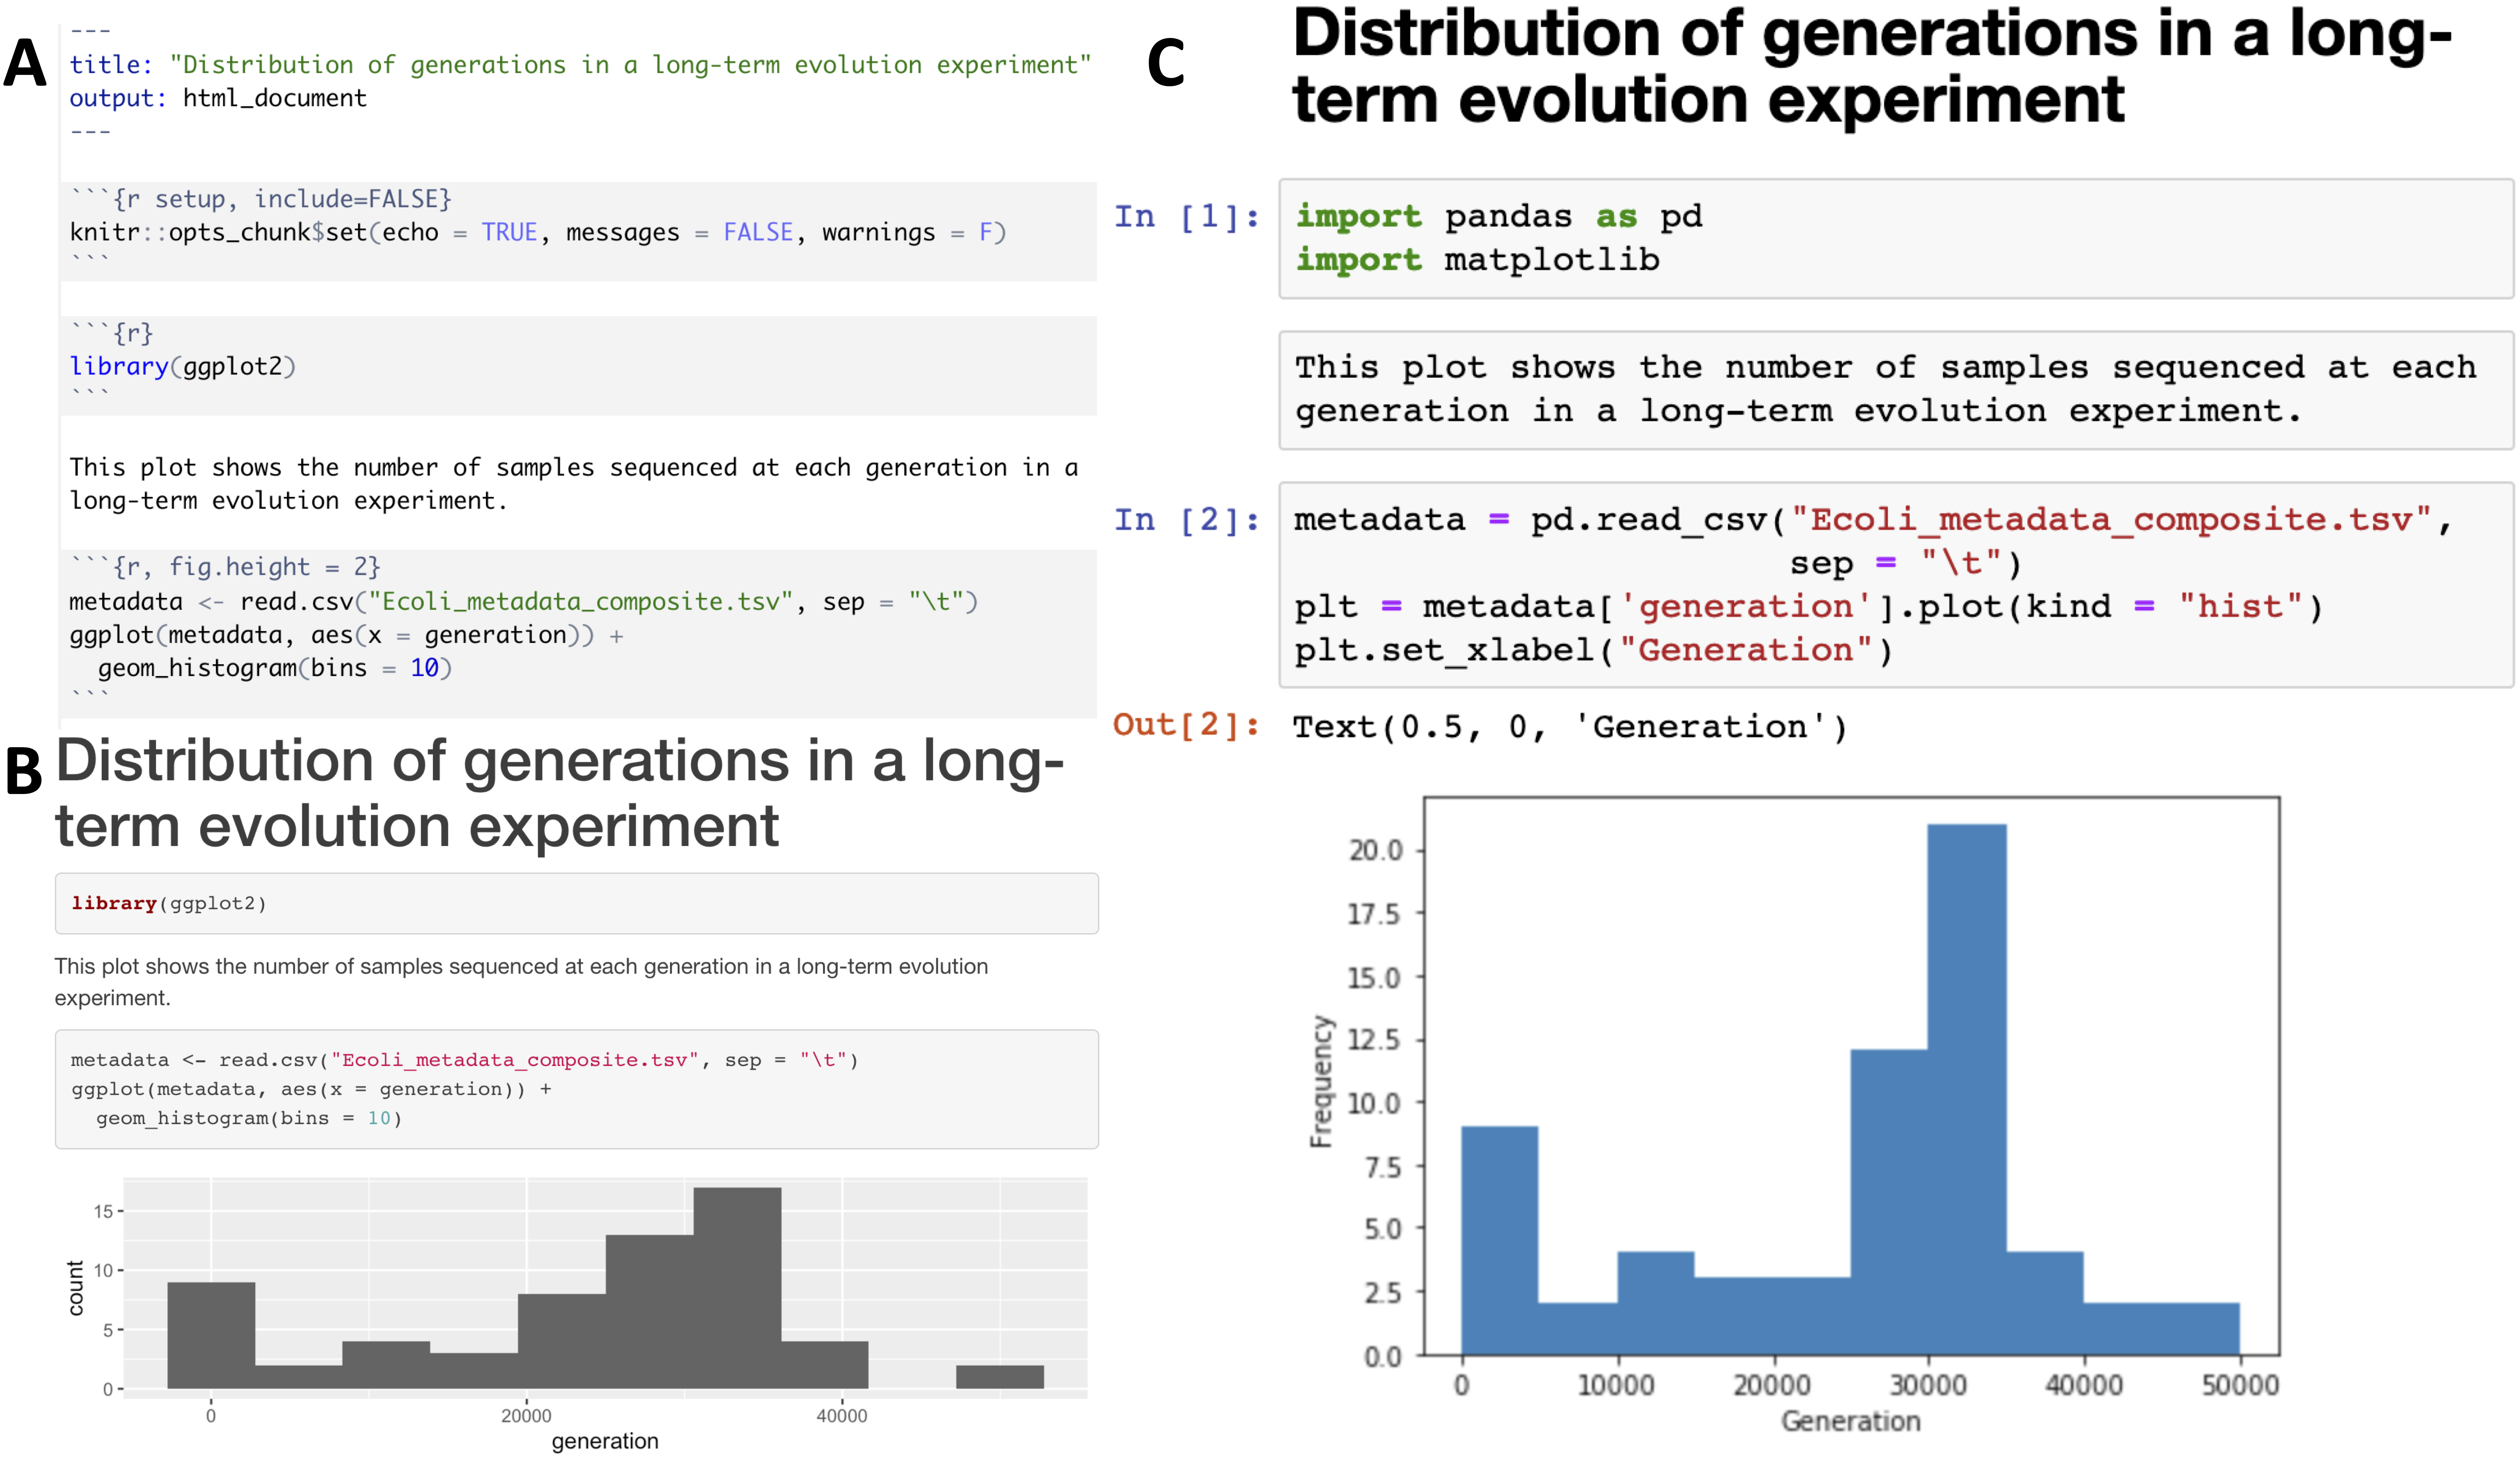
\includegraphics[width=0.99\textwidth]{figures/nb_figure.png}
\caption{Examples of computational notebooks. Computational notebooks allow the user to mix text, code, and results in one document. \textbf{A} shows a raw RMarkdown document viewed in the RStudio integrated development environment, while \textbf{B} shows a rendered HTML file produced by knitting the RMarkdown. \textbf{C} shows a Jupyter Notebook, where code, text, and results are rendered inline as each code chunk is executed. The second grey chunk is a raw markdown chunk with text that will be rendered inline when executed. Computational notebooks facilitate sharing by packaging narrative, code, and visualizations together.} 
\label{fig:nb_figure}
\end{figure}

 
\subsubsection*{Version Control} 

As your project develops, version control allows you to keep track of changes over time. 
You may already do this in some ways, perhaps with frequent hard drive backups or by manually saving different versions of the same file  - e.g. by appending the date to a script name or appending "version\_1" or "version\_FINAL" to a manuscript draft. 
For computational workflows that will inevitably undergo multiple changes in parameters, data, visualizations, and analysis, it is essential to keep track of which analysis produced which output files, so that the final analysis is reproducible. 
However, version control can also save time and effort at every step. 
If a key piece of a workflow inexplicably stops working, good version control can allow you to rewind in time and identify differences from when the pipeline worked to when it stopped working. 
If multiple people are working on the same project, version control can both avoid conflict and ensure that no productivity is lost. 

Version control systems such as Git or Mercurial can be used to properly keep track of all changes over time, even across multiple users, scripting languages, and including visualizations. 
In particular, Git has emerged as the dominant version control system for biological code, particularly when combined with online repositories such as Github, GitLab, or Bitbucket, which store online version histories for all tracked files.
In addition to acting as an additional backup location, the online services support drag-and-drop file addition and full control over the repository using the web interface, which greatly lowers the barrier to getting started with version control systems. 
While these systems do not work well with Google Docs or Microsoft Word, they can greatly simplify asynchronous collaborative manuscript writing when combined with services such as Overleaf and Manubot (CITE). 
Git version control is primarily designed to handle small text files, but version control also exists for data sets, since intermediate data files can change with tool versions or parameters. 
Many of the databases suggested for storing raw data also provide version control for data sets, including the Open Science Framework. 
Other services are compatible with git version control, e.g. Git Large File Storage (LFS) and Data Version Control (DVC).

These version control systems can also facilitate code availability and reproducibility for publication. 
For example, to ensure the correct version of the code is preserved, you can create a “release,” a snapshot of the current code and files in a GitHub repository. 
You can then generate a DOI for that release using Zenodo and make it available to reviewers and beyond (see "sharing" section, below).

%\begin{greybox}{git version control
%? do we even need this? probably not. will leave here in case we think of something to put in there.
%no - let's not talk about git code at all -- emphasize how easy the web interface is, and point people there
%until they feel the need to do things on the command line
%}
%\end{greybox}


\subsection*{Documenting reproducible workflows for yourself and others}

As with experimental biology, it is essential to write down everything you do - that is, record the origin of every file (e.g. download URL) and all metadata, record the version of software and each parameter you used, record any manual filtering or data preprocessing steps, and keep track of the order in which you executed each program. 
Without the ability to fully examine and reproduce your analysis, it will be impossible for you or your collaborators to assess whether the results are accurate, or even to understand how the heuristic decisions you took impact the conclusions made from an analysis. 

Computational project management is a learned skill that will take time to implement. There are a myriad of ways to document your computational work, and you'll need to experiment with the ways that work for you. 
For some portions of your project, you may want to document your work using a narrative approach, using written language to detail what steps you took and to communicate how the steps relate to one another. 
For other portions, it may be more useful to keep short, bulleted notes with your code or intersperse your commands with helpful diagrams. 
What is most important is to develop a clear documentation strategy and stick with it tenaciously. 
While the preferred tools discussed below will certainly change over time, these principles apply broadly and will help you design clear, well-documented, and reproducible analyses.
% Here are a few principles that apply broadly and may help you get started.

% current thinking: keep these principles short and general. Then put specific tools that will help with these below.
\subsubsection*{Use consistent and descriptive names}  
Consistent, descriptive names keep your project organized and interpretable for yourself and collaborators. 
This applies to your files, your scripts, your variables, your workflows, your manuscripts, and even your projects, each of which should have a unique and descriptive identifier. 
Since the number of files in data-intensive biology can quickly get out of hand, consistent file naming is especially important. 
For example, you can implement a numbering scheme for your files, where the first file in your analysis starts with "00", the next with "01", etc. 
You can also append the tool name to output to make it clear where the file came from. 
Additionally, using a standardized yet flexible folder structure from the outset of your project facilitates file organization, even as a project becomes increasingly complex. 
Keeping independent portions of your analysis in descriptive folders can help keep your project workspace clean and organized.
Within your files, using consistent and descriptive variable names will help build a readable codebase.

\subsubsection*{Store metadata information with your workflow} 
Biological analyses often span hundreds of steps and involve many small decisions: What parameters for each step? 
Why did you use a certain reference file for annotation as compared with other available files? 
How did you finally manage to get around the program or installation error? 
All of these pieces of information contextualize your results and may be helpful when writing your manuscript. 
Keeping information about these decisions in an intuitive and easily accessible place helps you find it when you need it. 
Each main directory should include notes on the data or scripts contained within, so that a collaborator could look into the directory and understand what to find there (especially since that collaborator is likely to be you, a few months from now!).
Code itself can be (or contain) documentation - you can add comments with the reasoning behind parameter choice or include a link to the seqanswers post that helped you decide how to shape your differential expression analysis. 
Larger pieces of information can be kept in ``README" or notes documents kept alongside your code and other documents. 
For example, a GitHub repository documenting the reanalysis of the Marine Microbial Eukaryote Transcriptome Sequencing Project uses a README alongside the code to document the workflow and digital object identifiers for data products (https://github.com/dib-lab/dib-MMETSP) \cite{johnson2019}.   
 %and liberal use of comments makes the purpose of specific lines of code explicitly clear.

\subsubsection*{Add visual representations} 
Visual representations illustrate the connections in a workflow. 
At the highest level, flowcharts that detail relationships between steps of a workflow can help provide big-picture clarification, especially when the pipeline is complicated. 
For individual steps, a graphical representation of the output can show the status of the project or provide insight on additional analyses that should be added. 
Whenever possible, adding visualizations can help improve the readability and reproducibility of your project. \textbf{Figure \ref{fig:sgc_workflow}} illustrates a workflow visualization modified from a graph produced by the workflow software Snakemake \cite{brown2019exploring}. 

\begin{figure}
\includegraphics[width=0.9\textwidth]{figures/hu_dag.png}
\caption{A directed acyclic graph that illustrates connections between all steps of a sequencing data analysis workflow. Each box represents a step in the workflow, while lines connect sequential steps.}
\label{fig:sgc_workflow}
\end{figure}

\subsubsection*{Sharing Your Reproducible Analyses} 
Sharing your workflow is a useful way to communicate every step you took in a data analysis pipeline. 
Your collaborators, peer reviewers, and scientists seeking to use a similar method as your own will all benefit from open and accessible code. 
Sticking to a clear documentation strategy, using a version control system, and packaging your code in notebooks or as a workflow prepare them to be easily shared with others. 
However, sharing code in this way can still be burdensome for others to interact with given the need for software installation and differences in user operating systems. 
Tools like Binder, Whole Tale, and Shiny apps can reduce the time to reproduction by other scientists by constructing controlled environments identical to those in which the original computation was performed. 
These tools substantially reduce overhead associated with interacting with someones code base and data, and in doing so, make it fast and easy to rerun portions of the analysis, check accuracy, or even tweak the analysis to produce new results. 
These tools are also great for teaching, as they provide consistent learner interfaces and environments. 

%TODO: first paragraph here should convey why sharing is important/great. We should assume not all folks reading this are on board with open everything (though we can try to convince them its the best way).

%Sharing can be very useful to share your workflow with collaborators (or peer reviewers!) so they can assess your steps... something about these tools making it very simple to run the code and check accuracy... Also great for teaching! So learning these will help on multiple fronts. 

%(poached from the version control section): You can also set use binder (mybinder.org) to make a running (containerized) version of this code (and visualizations) available,. [[See box for snakemake example. (same python/ bash/ graph as above? w/ conda installation) ** orrr link to example in workflow article? https://www.nature.com/articles/d41586-019-02619-z]]

\begin{greybox}{
 \textbf{Binder (mybinder.org)} Binder is a tool that makes a GitHub repository executable in a specified environment \cite{Jupyter2018}. 
It uses package management by R, pip, or conda to build a docker container with the software required to run the analyses contained in a GitHub repository. 
This is especially useful for computational notebooks. 
The binder can then be shared with collaborators (or students in a classroom setting), where the analysis or visualizations can be reproduced using your provided code. 
Binder instances are not static and can be modified by collaborators during a binder session. 
The underlying code will not be changed unless changes are committed into the original GitHub repository, preserving the reproducibility of the original analysis.
 
 \textbf{Shiny Apps} Shiny is a tool that allows you to build interactive web pages using R code. 
It allows you to package data that is manipulated  by R code in real-time in a web page, producing analysis and visualizations of a data set. 
Shiny apps can contain user-specifiable parameters, allowing a user to control visualizations or analyses. 
For example, if a Shiny app contained RNA-seq differential expression data, it might allow the user to specify which gene counts it should plot. 
Shiny apps allow collaborators who may or may not know R to change R visualisations to fit their interests.   
 
 \textbf{Other tools} There are many other tools that aid in reproducibility or sharing of results. 
Some tools, such as Whole Tale, aim to package the entire research object by capturing data, code and software environments in one executable package (CITATION). 
Other tools such as Vega-lite and plotly produce single interactive visualizations that can be shared with collaborators or integrated into websites (CITATIONS).
}
\end{greybox}

%\subsection*{Make big data less big} % heh. working title 
\subsection*{Scaling workflows} % some header that unites assessing required resources and comp approx.

\subsubsection*{Assess required resources}

Bioinformatic tools vary in the resources they require: some analysis steps are compute-intensive, other steps are memory intensive, and still others will have large intermediate storage needs. 
Tools will also vary in their ability to properly parallelize computation across multiple compute nodes. 
To minimize required computational resources for your analysis, it is worth assessing the resources required at each step.

Some tools publish required resources for test and sample data either in a publication or in software manuals or readmes. 
However if this information is not available, it's nearly impossible to estimate the amount of resources needed without running the tool. 
Monitoring resource usage (including RAM, CPUs, disk input and output, network usage, and time) while running the test data from a tool or on a subset of your data can give you a starting estimate for resource usage that you can scale up to accommodate the size of your actual data. 
Most workflow systems have built-in commands to report resource usage, while commands like ``time" and ``top" can show resource usage outisde of workflows.
Over time, you will develop an intuition for resource usage as you use more tools.

\subsubsection*{Scale workflows with tools that leverage computational approximations}
%\subsubsection*{Leverage computational approximations}
%\subsubsection*{Use computational approximations where possible}
 
 Many bioinformatics workflows take a long time and significant computational resources to run, and interpretable results are often only produced by the last few steps. 
This means that time-to-insight from sequencing data is often very high. 
 
Understanding the basic structure of data, the relationship between samples, and the approximate composition of each sample is very helpful at the beginning of data analysis, and can often drive analysis decisions in different directions than those originally intended. 
Although most bioinformatics workflows generate these types of insights, there are a few tools that do so rapidly, allowing the user to generate quick hypotheses that can be further tested by more extensive, fine-grained analyses. 

\textbf{Sketching} Sketching algorithms work with compressed approximate representations of sequencing data and thereby reduce runtimes and computational resources. 
These approximate representations retain enough information about the original sequence to recapitulate the main findings from many exact but computationally intensive workflows. 
Most sketching algorithms estimate sequence similarity in some way, allowing the user to gain insights from these comparisons.
For example, sketching algorithms can be used to estimate all-by-all sample similarity which can be visualized as a Principle Component Analysis or a multidimensional scaling plot, or can be used to build a phylogenetic tree with accurate topology. 
Sketching algorithms also dramatically reduce the runtime for comparisons against databases (e.g. all of GenBank), allowing users to quickly compare their data against large public databases. 
Sketching algorithms have been reviewed in-depth by Rowe \cite{rowe2019streaming}.

\textbf{Read quasi-mapping vs alignment} RNA-seq analysis approaches like differential expression or transcript clustering rely on transcript or gene counts.
Many tools can be used to generate these counts by quantifying the number of reads that overlap with each transcript or gene.
For example, tools like STAR and HISAT2 produce alignments that can be post-processed to generate per-transcript read counts.
However, these tools generate information-rich output, specifying per-base alignments for each read.
Quasi-mapping produces the minimum information necessary for read quantification, thereby reducing the time and resources needed to generate and store read count information (CITE: RAPMAP). 

\textbf{Anything else to mention?}  
+ blast approximations?


\section*{Practical considerations for workflow-enabled biology}

Your time and resources are valuable, and sequencing data analysis has the potential to use a lot of both. 
Leveraging publicly available data or using good experimental design sets an analysis up for success.
Conducting thorough quality control and workflow testing mitigates inefficiencies by helping you catch errors before they impact your full workflow or interpretation. 
Below we discuss some tips to ensure that you're spending your time and resources wisely. 

%\subsection*{Wrangling Sequence Data} % is "wrangling" too close to data carpentry?
\subsection*{Obtaining and maintaining quality data}
%\subsection*{Ensure you have quality data}

As with all biological analyses, a critical step of sequence analysis is obtaining high-quality data for your scientific question. 
With vast amounts of sequencing data already available in public repositories, it is often possible to begin investigating your research question by seeking out publicly available data. 
In some cases, these data will be sufficient to conduct your entire analysis. 
In others cases, particularly for biologists conducting novel experiments, these data can inform decisions about sequencing type, depth, and replication, and can help uncover potential pitfalls before they cost valuable time and resources.

\subsubsection*{Accessing publicly-available data}

Most journals now require data for all manuscripts to be made accessible, either at publication or after a short moratorium.
You can find relevant sequencing data either by starting from the ``data accessibility" sections of papers relevant to your research or by directly searching for your organism, environment, or treatment of choice in public data portals and repositories. 

The International Nucleotide Sequence Database Collaboration (INSDC), which includes the Sequence Read Archive (SRA), European Nucleotide Archive (ENA), and DataBank of Japan (DDBJ) is the largest repository for raw sequencing data. 
Additional curated databases focus on processed data instead, such as gene expression in the Gene Expression Omnibus (GEO).  
Organism-specific databases such as \textbf{Wormbase} (\textit{Caenorhabditis elegas}) specialize on curating and integrating sequencing and other data associated with a model organism \cite{harris2020wormbase}. 
The SRA, ENA, and DDBJ no longer accept raw sequencing data from large consortia projects, so data from these efforts are often hosted in consortia-specific databases such as those hosted by the Tara Ocean Foundation \cite{pesant2015open}.
Unlike the SRA and associated databases which are centralized and searchable, databases overseen by consortia often require domain-specific knowledge and have unique download and authentication protocols.
Finally, rather than focusing on certain data types or organisms, some repositories are designed to hold any data and metadata associated with a specific project or manuscript (e.g. Open Science Framework, Dryad, Zenodo \cite{foster2017open}).

%% a note about metadata for SRA, etc: https://www.embopress.org/doi/10.15252/embr.201745118

\subsubsection*{Generating your own data}
If generating your own data, proper experimental design and planning are essential. 
For cost-intensive sequencing data, there are a range of decisions about experimental design and sequencing (including sequencing type, sequencing depth per sample, and biological replication) that impact your ability to properly address your research question. 
These considerations will be different for different types of sequence analysis. 
While we have curated a series of domain-specific references that may be useful as go about designing your experiment (see \textbf{Table \ref{tab:seq_resources}}), conducting discussions with experienced bioinformaticians and statisticians, \textbf{prior to beginning your experiments} if possible, is the best way to ensure you will have sufficient statistical power to detect effects.
Given the resources invested in collecting samples for sequencing, it's important to build in a buffer to preserve your experimental design in the face of unexpected laboratory or technical issues. 

\begin{table}
\begin{tabular}{|c|c|}
\hline
\textbf{Sequencing type} & \textbf{Resources} \\
\hline
RNA-sequencing & \cite{conesa2016, schurch2016, ching2014} \\
\hline
Metagenomic sequencing & \cite{knight2012, quince2017, eisenhofer2019} \\
\hline
Amplicon sequencing & \cite{mclaren2019, murray2015, sinha2017 } \\
\hline
Microbial isolate sequencing & \cite{liao2015} \\
\hline
Eurkaryotic genome sequencing & \\
\hline
Whole-genome resequencing & \cite{fuentes2017} \\
\hline
Rad seq & \\
\hline
Chip seq & \\
\hline
ATAC seq & \\
\hline
single cell RNA-seq & \cite{bacher2016, haque2017} \\
\hline
? & \\
\hline
\end{tabular} 
\caption{\label{tab:seq_resources} References for experimental design and considerations for common sequencing chemistries.}
\end{table}

As your experiment progresses, keep track of as much information as possible -- dates and times of sample collection, storage, and extraction, sample names, aberrations that occurred during collection, kit lot used for extraction, and any other sample measurements you might be able to obtain (temperature, location, metabolite concentration, name of collector, etc). 
This metadata serves multiple purposes. 
First, it allows you to keep track of your samples and perform the experiments or comparisons you intended to perform. 
Second, it allows you to control for batch effects that may arise from unintended batching during sampling or experimental procedures. 
Third, recording more information may make the data you collect reusable for future applications and analysis by yourself and others, particularly for meta-analyses. 

\subsubsection*{Securing Computational Resources}

Sequence analysis requires access to computing systems with adequate storage and analysis power for your data. 
For some smaller-scale datasets, local desktop or even laptop systems can be sufficient, especially if using tools that implement data-reduction strategies such as minhashing \cite{rowe2019streaming}. 
However, larger projects require additional computing power, or may be restricted to certain operating systems (e.g. linux). 
For these projects, solutions range from research-focused high performance computing systems (e.g. university HPC, XSEDE/Jetstream, add non-USA example) to research-integrated commercial analysis platforms (e.g. AWS, Seven Bridges, Google Cloud, Microsoft Azure). 
Both research-only and  and commercial clusters provide avenues for research and educational proposals to enable access to their computing resources (see \textbf{Table \ref{tab:computational_resources}}). 
In preparing for data analysis, be sure to allocate sufficient computational resources and funding for storage and analysis, including large intermediate files and resources required for personnel training. 

\begin{table}
\resizebox{\textwidth}{!}{
\begin{tabular}{|c|c|c|}
\hline
Cloud Provider & Standard Model & Limits \\
\hline
Amazon Web Services & Paid & \\
\hline
Bionimbus Protected Data Cloud & Research allocation & users with eRA commons account \\
\hline
Cyverse Atmosphere & Free with limits & storage and compute hours \\
\hline
EGI federated cloud & Access by contact & European partner countries \\
\hline
Galaxy & Free with storage limits & data storage limits \\
\hline
Google Cloud Platform & Paid & \\
\hline
Google Colab & Free & computational notebooks, no resource guaruntees \\
\hline
Microsoft Azure & Paid & \\
\hline
NSF XSEDE & Research allocation & USA researchers or collaborators \\
\hline
Open Science Data Cloud & Research allocation & \\
\hline
Wasabi & Paid & data storage solution only \\
\hline
\end{tabular}}
\caption{\label{tab:computational_resources} \textbf{Research cloud resources} Cloud provider indicates the name of the cloud, standard model indicates the most common route toward using the cloud, and limitations indicates limitations in access or services provided by the cloud.}
\end{table}

%\begin{greybox}{\textbf{Research Cloud resources}
% 
%MAKE A TABLE, link to research proposal info (or payment info, I guess? Or just say "paid")!
%   - Galaxy
%   - XSEDE + Jetstream (USA; Research; examples of applications)
%   - cyverse
%   - AWS (Worldwide, Paid)
%   - https://www.opensciencedatacloud.org/
%   - google cloud https://www.blog.google/products/google-cloud/google-cloud-offers-global-support-for-academic-research/
%   }
% \end{greybox}


\subsubsection*{Storing data and metadata} %safeguard your data

As soon as you get your data, it is critical to store a read-only (write-protected) copy of your raw sequence files and any accompanying metadata (including experimental design, sequencing, and sample information) to safeguard against any accidental changes or deletions.
Ideally, keep one copy of the data in a location accessible to your computational workspace, and additional backups in different locations, such as \textit{both} a local backup disk and cloud storage.
Any changes you wish to make to your raw data during analysis (e.g. quality control) should be documented and saved to new files, rather than modifying the raw data. 
By ``keeping raw data raw", you'll be able to return to it anytime you need to change your workflow or develop a new analysis. 

When working with metadata, it may be necessary to reformat your files to facilitate computational analyses and comparisons between samples. In these cases, document the changes and store both the original files and the properly-formatted metadata as raw data. Standard guidelines for formatting data for scientific computing are given in \cite{wilson2017good}.

%Keeping metadata formatted in a way that is easy for a computer to interpret makes using the metadata easier for things like quality control or comparisons between samples.

\subsubsection*{Transferring Data (or not)} 

If your're working with publicly-available data, you may be able to work on a compute system where the data are already available, circumventing time and effort required for downloading and moving the data.
Databases such as the Sequence Read Archive (SRA) are now available on commercial cloud computing systems (Google, AWS; https://www.ncbi.nlm.nih.gov/sra/docs/sra-cloud/), and open source projects such as Galaxy enable import and work on SRA sequence files directly from a web browser (CITE galaxy, sra in cloud site). Ongoing projects such as the NIH Common Fund Data Ecosystem, aim to develop a data portal to make NIH Common Fund data, including biomedical sequencing data, more findable,
accessible, interoperable, and reusable (FAIR). 

In most cases, you'll still need to transfer some data - either downloading raw data or transferring important intermediate and results files for backup and sharing (or both). 
Checksums can be used to to check file integrity and ensure proper transfer (see \textbf{Figure \ref{fig:checksum}}).
File compression (gzip, bzip2, BAM/CRAM, etc.) can improve transfer speed and save space.
Tools like Rsync and Rclone automate file transfer between computers or between computers and remote storage providers \cite{bailleul2016rclone}. 
These tools automatically use checksums to verify that files were transferred properly.
Some GUI file transfer tools (e.g. cyberduck) also assess checksums when they are provided.

\begin{figure}
\centering

\includegraphics[width=0.75\textwidth]{figures/checksum.pdf}
\caption{\textbf{Use Checksums to ensure file integrity.} Checksum programs (e.g. md5, sha256) encode file size in a single value known as a ``checksum".
For any file, this value will be identical across platforms when calculated using the same checksum program. %hash algorithm. 
When transferring files, calculate the value of the checksum prior to transfer, and then again after transfer.
If the value is not identical, there was an error introduced during transfer (e.g. file truncation, etc).
For publicly-available files, a checksum value is often provided, so that you can check the integrity of the file after download.
 } 
\label{fig:checksum}
\end{figure}

\subsubsection*{Backup and storage} 
Many universities provide cloud storage space (e.g. through google drive, box, dropbox etc), and researchers can pay for individual storage on these services, or services attached to cloud computing (e.g. Amazon Web Services). 
Full computer backups can be conducted to these storage locations (e.g. with rclone \cite{bailleul2016rclone}), or there are also a number of paid services that will conduct backups at regular intervals (e.g. Backblaze, Dropbox Pro). 
There are also several free online repositories designed to help researchers store and share data and project materials. 
The Open Science Framework (OSF) \cite{foster2017open}, maintained and developed by the Center for Open Science, provides free storage of an unlimited number of files up to 5GB each in size, and allows the user to keep the data private until they are ready to share (make the project public). 
OSF provides built-in version control and is supported by a data preservation fund that will keep the data available for 50+ years. 
While OSF and other similar repositories (e.g. figshare) are suitable for use at any stage of a research project, repositories such as Zenodo and the Dryad Digital Repository (Dryad), are designed to make publication-ready data discoverable, citable, and reusable. 

% Link out to data/project management info? e.g. Many of these considerations are addressed in a data carpentry lesson (https://datacarpentry.org/organization-genomics/). 

%\subsubsection*{Compression for easier storage and transfer}
%Compression reduces the space needed to store files by encoding strings of characters in smaller representations. This not only saves storage space but also decreases the time required for data transfer. Many bioinformatic programs now work on either compressed and uncompressed data, meaning there is often no reason to fully uncompress data once compressed. Two types of compression are common in bioinformatics workflows: single file (e.g. data) compression, and archive compression. The most commonly-used single-file compression tool is gzip, which is often applied to fastq and fasta sequencing files (file suffix: `.gz`). Bzip2, which is gaining popularity as a gzip alternative, is more space efficient than gzip, but takes more time to compress files (though less time to decompress). The two most common archive compression, which combine many files into a single archive file, are tar (“tape archive”) and zip compression. These two types of compression can be combined for maximal compression: each file can be compressed before the archive file is generated, or the archive file itself can be compressed with gzip or bzip2. (best practice = the former?)

%\subsection*{Tools to facilitate documentation and reproducibility}



\subsection*{Ensure you have quality data} %purpose and strategies

%TODO: add punchy topic sentence on why QC is essential?
% TODO: reword QC section so organisation conveys:  (don't think we currently get these messages across)
 %- YOU are the best QC tool you've got. Look at / critically assess your data (at every step). Use that big brain for pattern recognition
% - Use visualization and tools to make this simpler! Hey, checkout out fastqc/etc in this greybox!
% - Here are some common errors and contaminants - make sure to look for them and other data-specific pitfalls
 
The adage, ``garbage in, garbage out" describes most sequencing data analysis: the quality of the input data determines the quality of the output results. 
Errors in sequencing data can be introduced at every stage, from sample generation to analysis. 
Assessing data at every analysis step can reveal these errors early. 
You are the single most effective quality control tool that you have, so its important to interrogate your data to search for problems. 
While simply looking at your data is sometimes sufficient to catch issues, visualization and software tools (e.g. FastQC, see \textbf{Figure \ref{fig:fastqc}}) make quality control easier. 

%% note on published data (from `accessing publicly-available data` section)
%As both sequencing technology and analysis tools have changed over time, we recommend conducting your own quality control upon beginning to work with a new dataset (see section \textbf{Quality  Control}).


\subsubsection*{Critically assess your data}
%\textbf{Look at your data} 
Quality control can be as simple as looking at the first few and last few lines of input and output data files, or checking the size of those files {\ref{tab:bash_commands}}. 
To develop an intuition for what proper inputs and outputs look like for a given tool, it is often helpful to first run the test example or data that is packaged with the software. 
Comparing these input and output file formats to your own data can help identify and address inconsistencies. 

Visualization is another powerful way to pick out unusual or unexpected patterns. 
Although large abnormalities may be clear from looking at files, others may be small and difficult to find. 
Visualizing raw sequencing data with FastQC (\textbf{Figure \ref{fig:fastqc}}) and processed sequencing data with tools like the Integrative Genome Browser and plotting tabular results files using python or R can make aberrant or inconsistent results easier to track down.

Many tools or operating systems generate log files or messages while running. 
These files contain information about the quantity, quality, and results from the run, or error messages about why a run failed. 
Inspecting these files can be helpful to make sure tools ran properly and consistently, or to debug failed runs. 
However, log files often contain voluminous text or special character spacing, making it difficult for both humans and computers to process the information therein. 
MultiQC is a helpful tool to parse and interpret some log files \cite{ewels2016}. 
MultiQC finds and automatically parses log files from other tools and generates a combined report and parsed data tables that include all samples. 
MultiQC currently supports 78 tools that span all stages of bioinformatic analysis pipelines, including all-star tools like samtools, BBMap, and FastQC. 

\begin{table}
\resizebox{\textwidth}{!}{
\begin{tabular}{|c|c|c|}
\hline
\textbf{command} & \textbf{function} & \textbf{example} \\
\hline
ls -lh & list files with information in a human-readable format & ls -lh *fastq.gz \\
\hline
head & print the first 6 lines of a file to standard out & head samples.csv \\
\hline
tail & print the last 6 lines of a file to standard out & tail samples.csv \\
\hline
less & show the contents of a file in a scrollable screen & less samples.csv \\
\hline
zless & show the contents of a gzipped file in a scrollable screen & zless sample1.fastq.gz \\
\hline
wc -l & count the number of lines in a file & wc -l ecoli.fasta \\
\hline
cat & print a file to standard out & cat samples.csv \\
\hline
grep & find matching text and print the line to standard out & grep ``\textgreater" ecoli.fasta \\
\hline
cut & cut columns from a table. & cut -d``," -f1 samples.csv \\
\hline
\end{tabular}}
\caption{\label{tab:bash_commands} Some bash commands are useful to quickly explore the contents of a file. By using these commands, the user can detect common formatting problems or other abnormalities.}
\end{table}


\begin{figure}
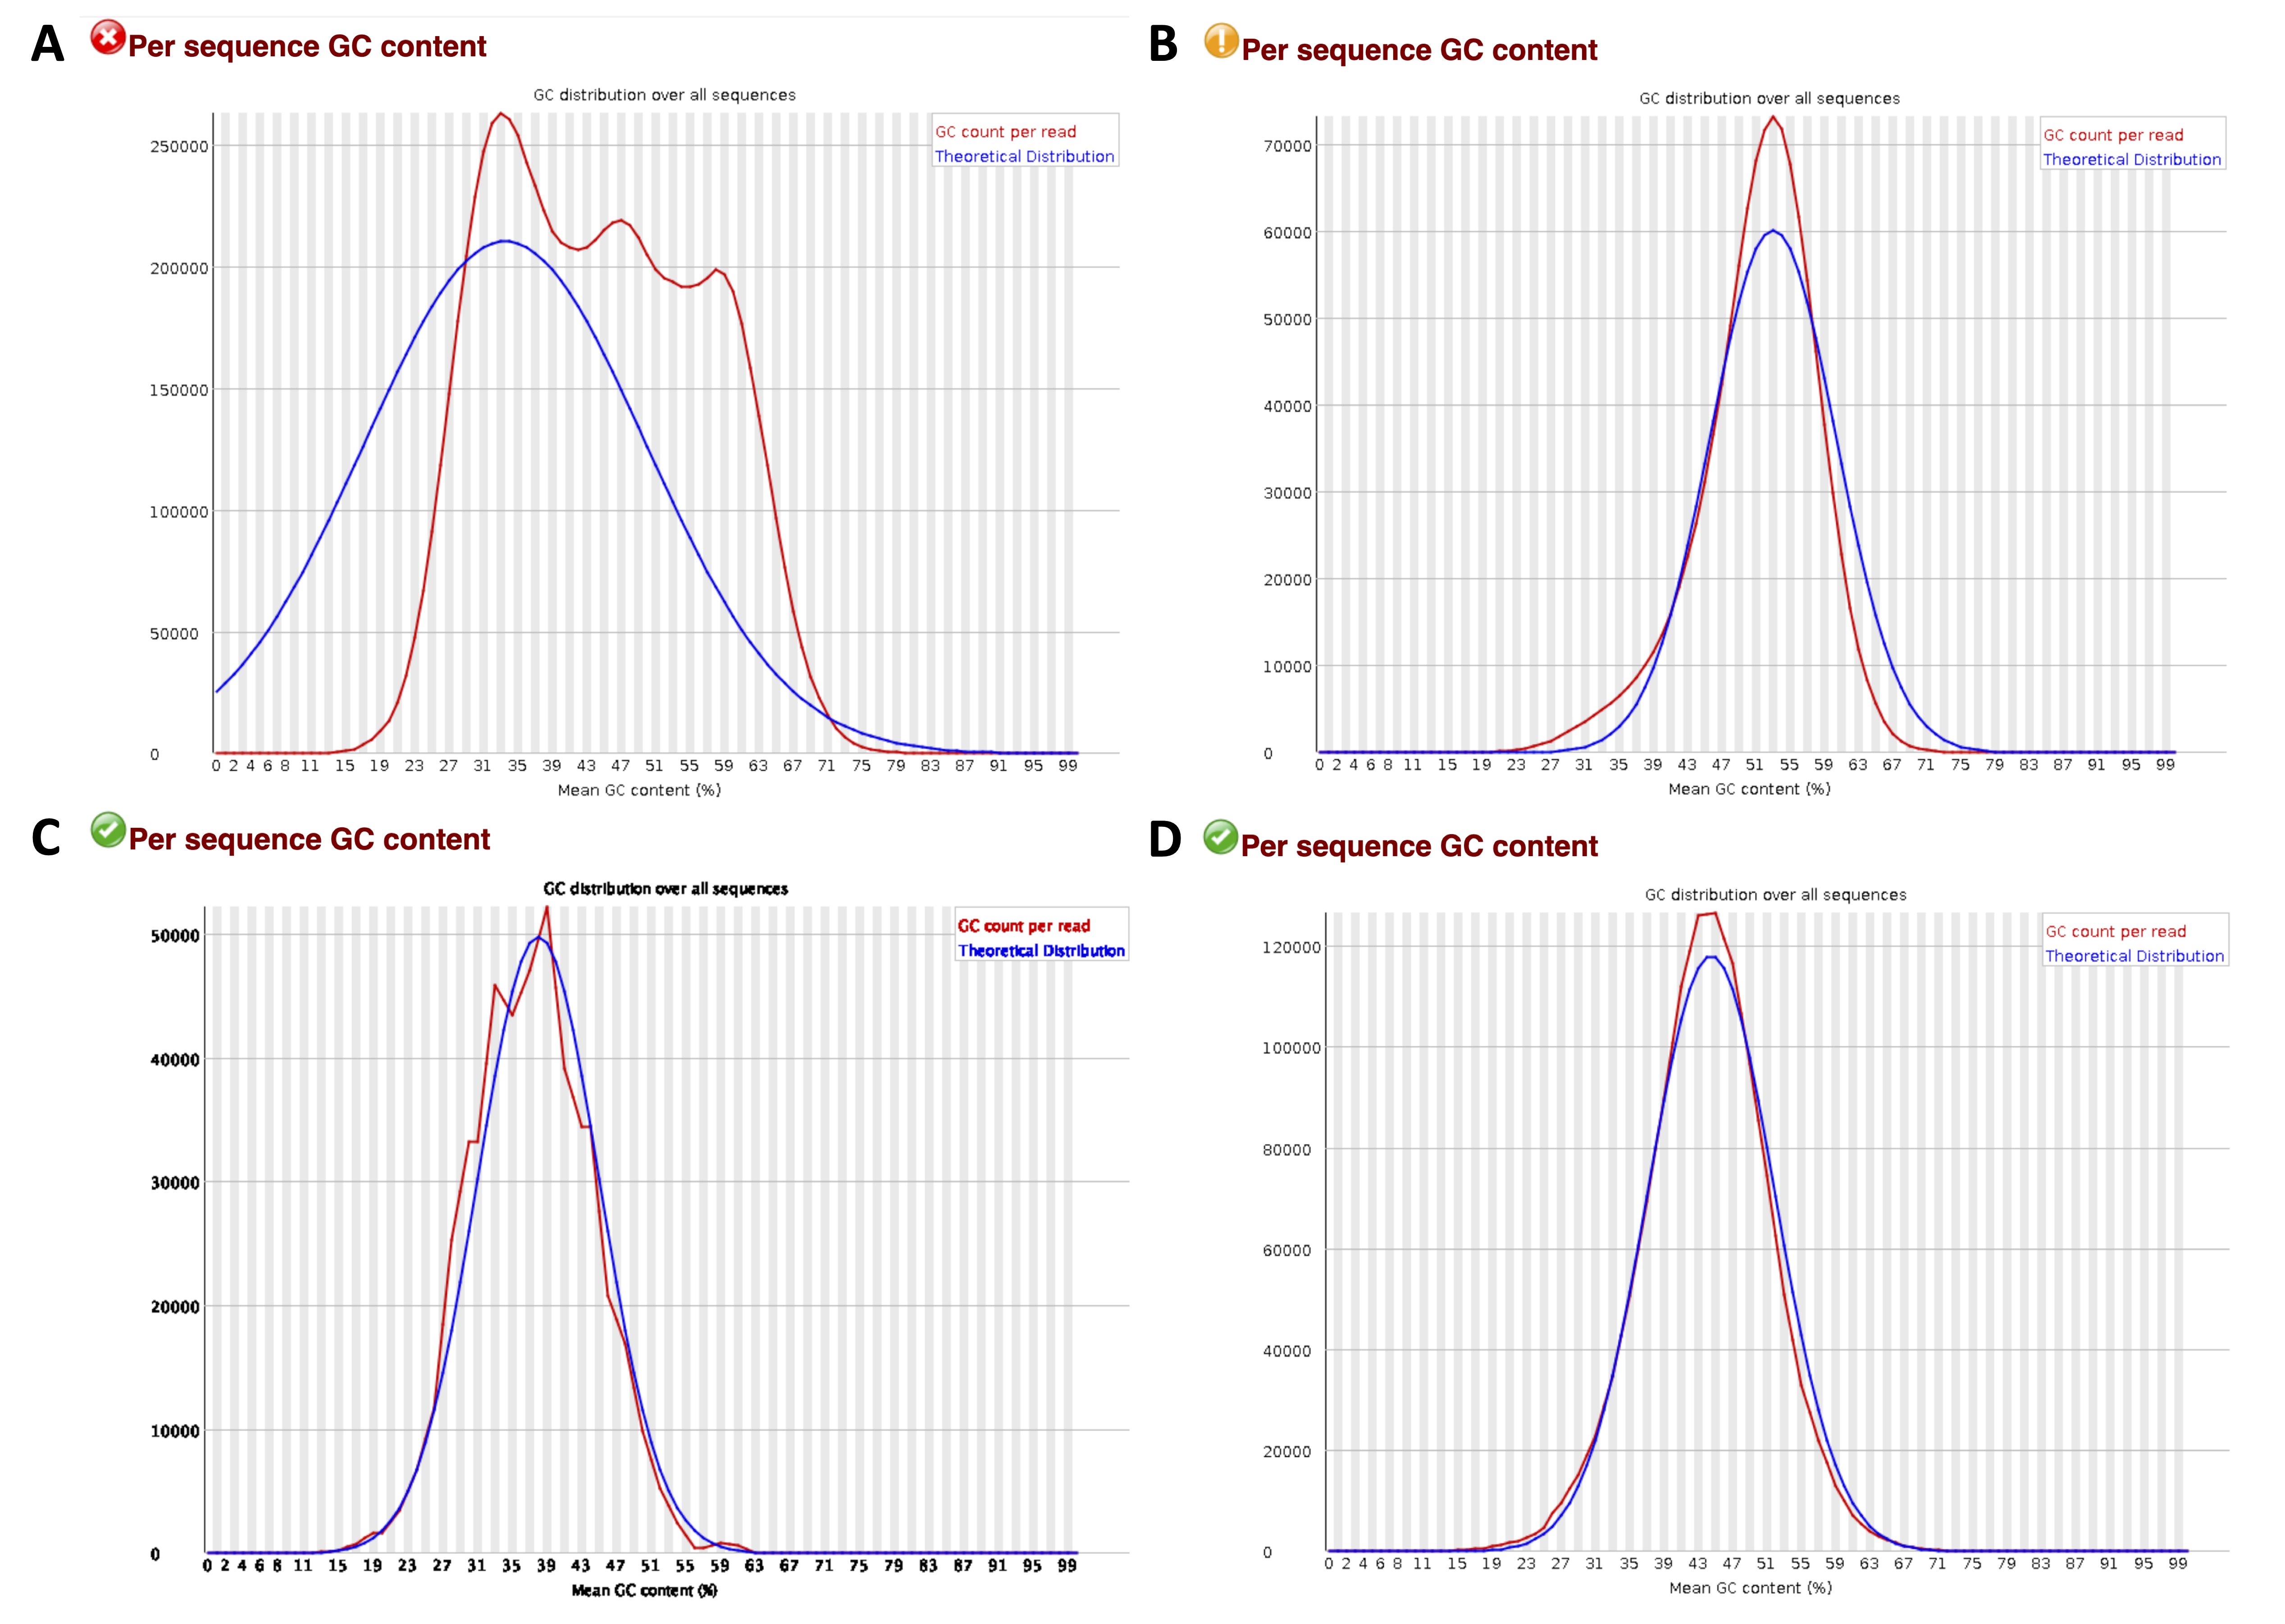
\includegraphics[width=.9\textwidth]{figures/fastqc.png}
\caption{FastQC provides quality control measurements and visualizations for raw sequencing data, and is a near-universal first step in sequencing data analysis because of the insights it provides.
FastQC measures and summarizes 10 quality metrics and provides recommendations for whether the sample is within an acceptable quality range. In this figure, we show the per sequence GC content quality metric for \textbf{A} a metagenome with bacteria and archaea species. \textbf{B} \textit{Escherichia coli} isolate genome sequencing, \textbf{C} RAD-sequencing and \textbf{D} RNA-sequencing from \textit{Saccharomyces cerevisiae}. While the GC distribution shown in \textbf{A} would be concerning if the sample were from an isolate, it is acceptable and expected to see non-normal distributions for metagenomes.} 
\label{fig:fastqc}
\end{figure}


%FastQC provides quality control measurements and visualizations for raw sequencing data, and is a near-universal first step in sequencing data analysis because of the insights it provides.
%FastQC measures and summarizes 10 quality metrics and provides recommendations for whether the sample is within an acceptable quality range. 
%The FastQC report is rich with information, both for prescribed and off-label interpretations. 
%For example, FastQC reports sequence length distribution, where the length of each read is plotted in a histogram. 
%For raw Illumina sequences, we expect a sharp peak where all reads are the same length; when there is variation in the length of sequences, we can infer that the reads have been trimmed in some way. 
%Another example is per sequence GC content. FastQC reports the percent content of GC nucleotides in the sequencing reads. 
%For single-species sequencing runs, we expect a smooth curve and a single peak. 
%If we observe multiple peaks, this may indicate that multiple species were sequenced in the sequencing run or that other abnormalities occurred during sequencing. 
%Many high-quality sequencing runs will fail FastQC metrics. 
%For example, we expect duplication levels to be high for RNA-sequencing or amplicon data. 
%Likewise, we expect multiple peaks in GC content for metagenomic data. 
%Insights gained using FastQC may not be definitive, but given the speed and computational tractability of the program, it is a rapid first-pass analysis to better understand the quality and content of the data that can be further tested by additional tools.}

\subsubsection*{Handling common biases in sequencing data} % this title isn't right yet, just trying to concisely summarize the all caps

There are many known biases in sequencing data. 
These biases originate from experimental design, methodology, sequencing chemistry, or workflows, and are helpful to target specifically with quality control measures. 
For example, PCR duplicates can cause problems in libraries that underwent an amplification step, and often need to be removed prior to downstream analysis. 
Contamination can arise during sample collection, nucleotide extraction, library prepartion, or through sequencing spike-ins like PhiX, and could change data interpretation if not removed (CITE TARDIGRADE PNAS PAPERS).
Libraries sequenced with high concentrations of free adapters or with low concentration samples may have increased barcode hopping, leading to contamination between samples (CITATION). 
Stringent trimming of RNA-sequencing data may reduce isoform discovery (CITE MCMANNES). 
The exact biases in a specific data set or workflow will vary greatly between experiments. 
To determine what issues are most likely to plague your specific data set, it can be helpful to find recent publications using a similar experimental design, or to speak with experts at a sequencing core.


Because sequencing data and applications are so diverse, there is no one-size-fits-all solution for quality control. 
Therefore, it is important to think critically about your expectations, and what patterns you expect to see given your data and your biological problem. 


\section*{Troubleshooting: how to help yourself and when to get help}

If you have tried the strategies above and are having trouble with your data, it’s time to ask for help. 
The first point of attack is always to Google the error, including any identifying error message or code, the program name, and if necessary, the type of data you’re running. 
There are a vast array of online resources for bioinformatic help ranging from question sites such as Stack Overflow and BioStars, to personal or academic blogs or even tutorials and lessons written by experts in the field. 
In most cases, the error you’ve encountered has been encountered many times before, and often the solution is readily available. 
If you can’t find any solutions in the relevant search results, it’s time to escalate. 
If the error is with a specific program, it’s best to post on that program’s help or issue location (e.g. GitHub Issues), or google group mailing list. 
Often the authors of your software will post their preferred location for answering questions and solving errors related to their program. 
Be sure to include the relevant details of your error, including terminal output and the version of the software you are using.
 If your error or question is more general, such as asking about program choice or workflows, Stack Overflow is a good choice. 
First, search through related topics to ensure your question has not already been answered. 
If it hasn’t, make a post to a relevant section, and be sure to include all relevant information in your post - type of data you have, approaches you’ve tried already, relevant error message, etc. 

While there is lots of help available online, there’s no substitute for local communities where you can get help working with your data and learning to troubleshoot. 
Many people around you may be experiencing similar issues and finding it difficult to find appropriate help. 
Developing a local bioinformatics community, either via seminar series or meetup sessions for data analysis, can also help in both improving and expanding your work in this area. 
Once you establish a local community, it may also be useful to set up a local online sites (e.g. discourse) for group troubleshooting. 
While this may seem like just a local version of Stack Overflow, the local, member-only nature can help create a safe and collaborative online space for troubleshooting problems often encountered by your local bioinformatics community. 
The benefit to beginners is clear: learning the best way to post questions and the important parts of errors, while getting their questions answered so they can move forward in their research. 
However, intermediate users may find these communities most useful, as they can also accelerate their own troubleshooting skills by helping others solve issues that they have already struggled through. 
While it can be helpful to have some “experts” available to help answer questions or to know when to escalate to Stack Overflow or other communities, a collaborative community of practice with members at all experience levels can help all its members move their science forward faster.


% For figure citations, please use "Fig" instead of "Figure".

%Nulla mi mi, Fig~\ref{fig1} venenatis sed ipsum varius, volutpat euismod diam. Proin rutrum vel massa non gravida. Quisque tempor sem et dignissim rutrum. Lorem ipsum dolor sit amet, consectetur adipiscing elit. Morbi at justo vitae nulla elementum commodo eu id massa. In vitae diam ac augue semper tincidunt eu ut eros. Fusce fringilla erat porttitor lectus cursus, \nameref{S1_Video} vel sagittis arcu lobortis. Aliquam in enim semper, aliquam massa id, cursus neque. Praesent faucibus semper libero.

% Place figure captions after the first paragraph in which they are cited.
%\begin{figure}[!h]
%\caption{{\bf Bold the figure title.}
%Figure caption text here, please use this space for the figure panel descriptions instead of using subfigure commands. A: Lorem ipsum dolor sit amet. B: Consectetur adipiscing elit.}
%\label{fig1}
%\end{figure}

% Results and Discussion can be combined.
%\section*{Results}
%Nulla mi mi, venenatis sed ipsum varius, Table~\ref{table1} volutpat euismod diam. Proin rutrum vel massa non gravida. Quisque tempor sem et dignissim rutrum. Lorem ipsum dolor sit amet, consectetur adipiscing elit. Morbi at justo vitae nulla elementum commodo eu id massa. In vitae diam ac augue semper tincidunt eu ut eros. Fusce fringilla erat porttitor lectus cursus, vel sagittis arcu lobortis. Aliquam in enim semper, aliquam massa id, cursus neque. Praesent faucibus semper libero.


%PLOS does not support heading levels beyond the 3rd (no 4th level headings).
%\subsection*{\lorem\ and \ipsum\ nunc blandit a tortor}
%\subsubsection*{3rd level heading} 
%Maecenas convallis mauris sit amet sem ultrices gravida. Etiam eget sapien nibh. Sed ac ipsum eget enim egestas ullamcorper nec euismod ligula. Curabitur fringilla pulvinar lectus consectetur pellentesque. Quisque augue sem, tincidunt sit amet feugiat eget, ullamcorper sed velit. Sed non aliquet felis. Lorem ipsum dolor sit amet, consectetur adipiscing elit. Mauris commodo justo ac dui pretium imperdiet. Sed suscipit iaculis mi at feugiat. 

%\begin{enumerate}
%	\item{react}
%	\item{diffuse free particles}
%	\item{increment time by dt and go to 1}
%\end{enumerate}

%\begin{itemize}
%	\item First bulleted item.
%	\item Second bulleted item.
%	\item Third bulleted item.
%\end{itemize}

\section*{Conclusion}

%CO\textsubscript{2} 
% For more information, see \nameref{S1_Appendix}.

\section*{Supporting information}

% Include only the SI item label in the paragraph heading. Use the \nameref{label} command to cite SI items in the text.
%\paragraph*{S1 Fig.}
%\label{S1_Fig}
%{\bf Bold the title sentence.} Add descriptive text after the title of the item (optional).

%\paragraph*{S2 Fig.}
%\label{S2_Fig}
%{\bf Lorem ipsum.} Maecenas convallis mauris sit amet sem ultrices gravida. Etiam eget sapien nibh. Sed ac ipsum eget enim egestas ullamcorper nec euismod ligula. Curabitur fringilla pulvinar lectus consectetur pellentesque.

%\paragraph*{S1 File.}
%\label{S1_File}
%{\bf Lorem ipsum.}  Maecenas convallis mauris sit amet sem ultrices gravida. Etiam eget sapien nibh. Sed ac ipsum eget enim egestas ullamcorper nec euismod ligula. Curabitur fringilla pulvinar lectus consectetur pellentesque.

%\paragraph*{S1 Video.}
%\label{S1_Video}
%{\bf Lorem ipsum.}  Maecenas convallis mauris sit amet sem ultrices gravida. Etiam eget sapien nibh. Sed ac ipsum eget enim egestas ullamcorper nec euismod ligula. Curabitur fringilla pulvinar lectus consectetur pellentesque.

%\paragraph*{S1 Appendix.}
%\label{S1_Appendix}
%{\bf Lorem ipsum.} Maecenas convallis mauris sit amet sem ultrices gravida. Etiam eget sapien nibh. Sed ac ipsum eget enim egestas ullamcorper nec euismod ligula. Curabitur fringilla pulvinar lectus consectetur pellentesque.

%\paragraph*{S1 Table.}
%\label{S1_Table}
%{\bf Lorem ipsum.} Maecenas convallis mauris sit amet sem ultrices gravida. Etiam eget sapien nibh. Sed ac ipsum eget enim egestas ullamcorper nec euismod ligula. Curabitur fringilla pulvinar lectus consectetur pellentesque.

\section*{Acknowledgments}
thanks thanks thanks thanks

\nolinenumbers

% Either type in your references using
% \begin{thebibliography}{}
% \bibitem{}
% Text
% \end{thebibliography}
%
% or
%
% Compile your BiBTeX database using our plos2015.bst
% style file and paste the contents of your .bbl file
% here. See http://journals.plos.org/plosone/s/latex for 
% step-by-step instructions.
% 

% this compiles our bibliography.bib file and inserts references here
%not sure if we need to paste refs in prior to submission, see http://journals.plos.org/plosone/s/latex
\bibliography{bibliography}

\end{document}
